\documentclass[10pt,a4paper,usenatbib]{article}
\usepackage[utf8]{inputenc}
\usepackage[english]{babel}
\usepackage[round]{natbib}
\usepackage{amsmath}
\usepackage{amsfonts}
\usepackage{amssymb}
\usepackage{graphicx}
\usepackage{wrapfig}

\newcommand{\fpath}{./Figs/}

\begin{document}
\title{A Multi Agent System for the Modellization of the Rationality of People's Decisions in a Peer to Peer Environment}

\author{Kim Nicoli, Francesco Parino, Luca Rickler}
\date{19 July 2016}
\maketitle
\pagebreak

\tableofcontents

\pagebreak


\section{Introduction}


\subsection{General Overview}

The subject we present in this paper has originally been inspired
by the Kolkata Paise Restaurant problem; more in detail we took inspiration
from the paper \textit{\textquotedblleft The Kolkata Paise Restaurant
Problem and Resource Utilization\textquotedblright} by \citet{Chakrabarti2009}. 

The problem mentioned in the paper is modelled as a One-Shot game
which takes place in Kolkata, the Indian capital of West Bengal, where
there are many cheap and fixed rate restaurants usually frequented
by workers at lunch time.

In order to save the transport costs, people usually walk down to
one of these cheap restaurants to have lunch during their lunch break.
So, here is the problem: every single restaurant's capacity to serve
customers is limited, and every diner will not serve more than a fixed
number of customers on each day. As a matter of fact, if most of the
workers go to the same restaurant, this will not be able to satisfy
every one of them and some will not get lunch and consequently will
go back to work hungry and unsatisfied.

Moreover, if someone goes to an already filled restaurant, then walking
down to another restaurant would mean failing to report back to work
in time. It is even important to underline that in the classic version
of the problem there is the assumption that every restaurant serves
lunches of different qualities - according to a ranking known to the
customers - but that the prices are the same anywhere, no matter how
high the quality of the restaurant is.

The problem is quite simple to understand, but, on the other hand,
is quite difficult to be solved. It is obvious to imagine that every
worker possibly wants to go to the best ranked restaurant in Kolkata
and be served. In light of what we saw before, this is unrealistic
because the capacity of every restaurant is limited; maybe one restaurant
can serve more than one customer each day, but will not be able to
satisfy all the workers of the city.

The Kolkata Paise Restaurant problem can be seen as a complication
of the El Farol bar problem, a problem in game-theory based on a bar
in Santa Fe, New Mexico, created in 1994 \citep[Arthur, ][]{arthur1994} but, in fact, formulated
and solved six years earlier, in 1988, with a different name. Here we will face the problem by using the multi-agent
modelling technique.


\subsection{Solving the problem through a MAS model}

This problem has already been modelled by an Agent Based Model (ABM)
project, written in Netlogo, where smart agents tried to find the
best strategy in order to maximize their own satisfaction, without
communication with other people. 

Now, our aim is to bring the problem on an upper level by modelling
a similar situation through a Multi Agent System (MAS) project, which
is quite different. Where we had smart agents acting on their own,
now we have agents who interact among them by the introduction of
a mutual communication. Although agents are not as intelligent as
they were in the ABM model, now they can communicate and bring out
a collective intelligence through out their social behaviour, led
by their interaction.

The main target of this work is to outline how the communication among
agents at a very low level could influence the rise of a collective
behaviour.

It is even important to underline that the problem studied by \citet{Chakrabarti2009} was a One-Shot Game. Hence,
we had \emph{One-Shot behaviours} which means that people just act
once in looking for an available restaurant\footnote{in the paper authors assumed that every restaurant had just one place
available.}, if they fail (don't find a good restaurant) they immediately stop. 

Our situation is far more different; we have to deal with \emph{cyclic
behaviours}. Every agent has a protocol to follow and a list of task
predicates to satisfy; thus, if he does not find a restaurant at the
first attempt he tries again with another one, until he find a place
with available tables or he realises, after having checked all restaurants,
that there are no tables available anywhere so that the task can not
be satisfied.

Furthermore, the MAS solution we are going to describe is similar to a \textit{peer to peer} communication network, as every person knows and talks to only a small segment of the whole population (her friends) sending small chunks of information.

\section{Model Design}


\subsection{Agent types and hierarchy}

We have basically two type of agents: People and Restaurants.

People are more dynamical agents since they take decisions, continuously
update their knowledge database and contribute to modify the external
environment.

Moreover, they hold many different characteristics.

\emph{boldness}, a \emph{minimum evaluation} and a \emph{list of friends}. 
\begin{itemize}
\item ``\emph{Boldness}'' referrers to the attitude of the agent to learn
from what he experienced. That means if he had a bad experience in
a certain restaurant if his boldness is low he would not return there
again, while, if is boldness is high, he would probably give to the
restaurant a second chance. 
\item The \emph{minimum evaluation} referrers to the lowest restaurant quality
a person is minded to accept. A high value of this parameter represents a very exigent customer while
a low one will lead the agent anywhere, no matter the quality of the food. In our simulations we kept this parameter fixed to zero to avoid having very exigent customers and focus more on the overall behaviour of the population.
\item The last parameter, is the \emph{list of friends} that every person
has; these friends could influence the thought of a single agent by
communicating him their thinking. Every agent, for each one of his
friends, has an attribute which is the ``\emph{trust}'' that this
person put in all of them; we could say, in this sense, that my best
friend is the one I believe the most.
\end{itemize}
On the other hand, restaurants are more simple than people. As a matter
of fact, we have only two parameters to deal with: the \textit{capacity} and the
\textit{rank}.
\begin{itemize}
\item As we could expect a single restaurant could not serve everyone; that's
the reason why we need a\emph{ capacity}. Once a restaurant is filled
it can not accept other bookings. So people who expected to go there
need to change their goal. 
\item The second parameter, \emph{the rank}, outlines the objective quality
of a restaurant. We fixed an evaluate range from $0$ to $5$, where five
means best quality restaurants while zero are the worst ones.
\end{itemize}

\subsection{Model Work-flow}

The structure of the communication is quite simple. As mentioned before
we treat the problem differently from \citet{Chakrabarti2009}. In our analysis
we have to deal with a Repeated-Game instead of a One-Shot Game (which
is far more abridging).

We organised our protocol in turns. For each turn, every single person
follows a precise sequence of actions:
\begin{itemize}
\item\textit{Search}: first of all, an agent needs to find among all
restaurants the one which is the best for him.
\item\textit{Choose}: secondly he must control that this restaurant has
available places; thus, if the best restaurant is already full he
goes for the second and so on.
\item\textit{Eat}: then, once he found a good restaurant to book at,
he goes there and eats.
\item\textit{Evaluate}: finally, the agent updates his own opinion of
the restaurant, for the next turn, grounding on what he experienced.
\end{itemize}
This protocol will be explained in a more detailed way later in section \ref{subsec:comm_protocol}.


\subsection{Strategies}
\label{subsec:strategies}
The action of choosing the best restaurant is an interesting and important
thing to analyse. In this sense, we select two main strategies that
an agent can follow in choosing the best place to eat. It is important
to underline that the probability a single customer chooses one strategy
instead of another can be set before launching the simulation.

The strategies we consider are:
\begin{itemize}
\item\textit{Rational Choose}: this is the most common way of choosing.
The customer selects all restaurants that satisfies his \emph{maximum
evaluation}, and among them chooses the best one which has available
places.
\item\textit{Irrational Choose}: the second strategy brings to our model
some fuzzy logic through an irrational way of choosing. As a matter
of fact an agent chooses at random, among the restaurants that have
available places, where to go.
%\item\textit{Best Friend Choose}: the third strategy is probably the
%most interesting to outline the influence of the communication between
%people in our model. In this strategy a person decides to go to the
%restaurant which is thought the best one by the friend in which he
%believes the most (his \emph{best friend}!). Obviously, if the restaurant
%is already full, the agent will go for the second preference of his
%best friend ``top ranked restaurants'' and so on, until he finds
%the best restaurant with available places.
\end{itemize}

\pagebreak

\section{Implementation}
\label{sec:implementation}
We wrote the model in Java, using the JADE\footnote{\textbf{www.jade.tilab.com}} library, developed by Telecom Italia Lab. We chose it because it offers a range of agent and behaviour types as well as a built-in support for communication between agents.

For the generation of random numbers, we used the uniform distribution RNG built in the Java standard library.

We also implemented the option to load the simulation set-up, including all randomly generated quantities, from a JSON file generated during another simulation. When this feature is used, the JSON data is distributed   to each agent during the initialization phase.
\subsection{Classes overview}
The model is mainly composed of two type of classes: agents and behaviours. 
Besides the person and restaurant type of agents, we implemented a third type called global. This is responsible for the simulation initialization and turn structure and is better described in section \ref{subsec:global}.

Each of these three type of agents has access to its own set of behaviours. Each of this is composed by a message receiver, implemented as a \textit{cyclic behaviour}, a type of behaviour that is always scheduled for execution after its completion, and several \textit{one-shot behaviours}, which are not rescheduled after completion. The most simple \textit{one-shot behaviour} is a message sender, present in the restaurant and global set of behaviours. Person has several more complex behaviours, better described in section \ref{subsec:person}

\subsection{Communication protocols}
\label{subsec:comm_protocol}
The main communication protocol we designed is the one responsible for the interaction between people and restaurants, which is shown in figure \ref{fig:comm_protocol}. The communication is started by a person agent, which sends a \textit{Request} to the restaurant. If the restaurant is already full, it will answer with a \textit{Refuse}, ending the communication. Otherwise, it will answer with a \textit{Propose}. Normally, the same person sends many requests at once to different restaurants. After receiving all the answers, the person agent chooses the best restaurant according to one of the strategies previously described in section \ref{subsec:strategies}. The person, then, sends an \textit{Accept Proposal} to this restaurant, which in turn checks again how much space left it has. If there's none, it will send a \textit{Failure} and the communication will end. This may happen in case of slow communications and concurrent actions by many people. If instead it still has some space left, it will send the person an \textit{Inform} containing it's quality and set the seat as occupied. This ends the communication. 
\begin{figure}
\includegraphics[width=11cm]{\fpath/CommunicationPR_mk2.png}
\caption{\small \textit{Diagram of the communication protocol between people and restaurants}}
\label{fig:comm_protocol}
\end{figure}

\pagebreak

\subsection{Global}
\label{subsec:global}
To control the turn structure and initialize the model, we implemented a third type of agent called global. 

\begin{wrapfigure}{l}{0.5\textwidth}
\centering
\includegraphics[width=4cm]{\fpath/Global_General.png}
\caption{\small \textit{Diagram of the internal logic of the Global class}}
\label{fig:global_flow_big}
\end{wrapfigure}

Figure \ref{fig:global_flow_big} shows the internal logic of the global agent. This can be divided in three phases (blue boxes) and some other actions. At first, the global agent initializes, randomly or with preloaded JSON data, all the other agents and collects their data in JSON format. At the end of this first phase, it saves the JSON configuration files. Then, it signals the restaurants to reset and waits for their answer. At last, it notifies the start of the turn to the people. At the end of the turn, each person sends its data to the global agent. This turn sequence is repeated for a fixed number of time steps, chosen at the start of the simulation.
At the end of the last turn, the global agent saves on disk the log files containing all the data of the simulation.

\begin{wrapfigure}{r}{0.5\textwidth}
\centering
\includegraphics[width=3cm]{\fpath/Global_specific.png}
\caption{\small \textit{Diagram of the internal logic of a phase of the Global class logic}}
\label{fig:global_flow_small}
\end{wrapfigure}

The internal structure of a single phase is shown in figure \ref{fig:global_flow_small}. Each starts with a \textit{Confirm} performative broadcast to all the agents which signals the beginning of the phase. The different phases are distinguished through the message ontology. The phase ends when the global agent has received an answer from all the agents involved containing the results of the computation.
%Then the Global agent listens for incoming messages with the result of the computation for that phase till it has received an answer from all the interested agents. 


\pagebreak

\subsection{Restaurant}
The restaurant agents work as an automatic answerer: their only task is to answer to incoming questions asked by the other agents. Their two parameters, capacity and quality, are randomly generated in a specified range on initialization.

As figure \ref{fig:restaurant_flow} shows, the internal logic of the restaurant agents is rather simple: they listen to incoming messages and answer based on the message performative. If the message performative is \textit{Request}, the restaurant checks for free space and answers with a \textit{Propose} if there is any or a \textit{Refuse} if there is none. This is the first phase of the person-restaurant communication protocol.

On an \textit{Accept Proposal}, it will again check for free space and answer with an \textit{Inform} containing its quality if there is still unoccupied space or a \textit{Failure} if there is none. This is the second phase of the person-restaurant communication protocol. 

At last, if the message performative is \textit{Confirm}, it will answer with a propagate only if the message ontology is "reset", which corresponds to the restaurant reset phase in the turn structure.
\begin{figure}
\includegraphics[width=10cm]{\fpath/Restaurant.png}
\caption{\small \textit{Diagram of the internal logic of the Restaurant class}}
\label{fig:restaurant_flow}
\end{figure}

\pagebreak

\subsection{Person}
\label{subsec:person}
Unlike the restaurants, the person agents play a more active role in the simulation: as it has been said earlier, they have the ability to take decisions and have a personal opinion regarding the environment in the form of a knowledge database.

The three properties of each person agent, \textit{boldness}, \textit{maximum evaluation} and its \textit{list of friends} are randomly generate on initialization. Their range is set at the start of the simulation.

\begin{wrapfigure}{r}{0.5\textwidth}
\centering
\includegraphics[width=4cm]{\fpath/Person_General.png}
\caption{\small \textit{Diagram of the internal logic of the Person class}}
\label{fig:person_flow}
\end{wrapfigure}

Figure \ref{fig:person_flow} shows the internal logic of a person agent. After the global initialization phase, described in section \ref{subsec:global}, the agent waits for the broadcast announcing the start of the turn. Afterwards, it starts the \textit{search} routine: it sends a \textit{Request} message to every restaurant which it thinks to be better than its \textit{maximum evaluation} parameter. Then it collects all the answers, selecting only the positive ones, containing a \textit{Propose}, and starts the \textit{choose} routine. At this point, it selects randomly one of the two strategies described in section \ref{subsec:strategies}. The probabilities with which it will select one of them is set at the start of the simulation. Using one of these strategies, the agent selects the best restaurant and sends it an \textit{Accept proposal} with its \textit{eat} routine. If somehow, in the meantime, the restaurant has received enough bookings to fill all the available tables, it replies with a \textit{Failure} and the person will start again the whole search process excluding the previously chosen restaurant from its search list. Otherwise, the restaurant replies with an \textit{Inform} containing its effective quality. The person then compares this with the restaurant record in its knowledge database and update the latter with the \textit{evaluate} routine. The update rule is better described in section \ref{subsec:eval_update_rule}. At last, the person sends its new evaluation to its friends, who will use it to update their trust-map when they will eat in the same restaurant with the following rule

\begin{equation*}
T' = 1 - \frac {\vert\Delta Q\vert}{R} 
\end{equation*}

where $T$ is the friend's new trust, $\Delta Q$ is the difference in evaluation with the person's, $R$ is the evaluation range, set to $5$. This is then mediated with the old trust value.
The person agent then notifies the global agent the end of its turn.

\section{Analysis}
In the first part of this chapter we introduce some theoretical arguments useful in the analysis. Then, we start considering a basic version of the model, trying to understand the basic concepts and ensure that everything works fine. Successively, we try to explain what are the consequences of a specific agent's behaviour and analysing some aspects of the entire model.   

We analysed the simulation data with an iPython notebook we wrote, using the Pandas, Numpy and Matplotlib libraries.

\subsection{Evaluation update}
\label{subsec:eval_update_rule}
Analysing how people update their knowledge database, we can find an exponential law.\\
Let $B$ be the agent's boldness, $Q$ the real quality of a restaurant and $V$ the internal evaluation regarding that restaurant. \\   
Thought by the agent on his own, people update $V$ step by step with the following recursion rule
\[V\left( {t + 1} \right) = V\left( t \right) + B\left( {Q - V\left( t \right)} \right)\]
by considering an infinitesimal time step $dt$ we can look at this relation as a derivative that we could integrate 
\[\frac{1}{B}\frac{{dV}}{{dt}} = Q - V\left( t \right)\]
In light of this, we obtain both an homogeneous solution:
\[\begin{array}{l}
\frac{1}{B}\frac{{dV}}{{dt}} =  - V\left( t \right)\\ \\
V\left( t \right) = V\left( 0 \right){e^{ - Bt}}
\end{array}\]	
And a particular one:
\[V\left( t \right) = Q\]
Thus, the complete solution of this partial differential equation will be the following
\[\boxed{V\left( t \right) = {V_0}{e^{-Bt}} + Q}\]


\subsection{Analysing the global knowledge}
Let’s now analyse the model on what concerns the global knowledge related to all agents about restaurant’s quality. As mentioned before each restaurant is characterized by a particular ranking value which outlines its quality. Moreover, the ranking is actually a dual variable: there’s the Real ranking $Q$ unknown to customers and the personal thinking, for each person, of restaurant’s quality, $V$; this ranking is, thus, strictly related to the agent’s knowledge database.\\
Thus, we introduce for, each restaurant, an uncertainty factor $K_{re}$ which is defined as the variance of the evaluation of all the people at the specific time step $t$:

\begin{equation}
  {K_{re}}\left( t \right) = {\sum\limits_{per} {\left( {\mu \left( t \right) - {V_{re,per}}\left( t \right)} \right)} ^2}
\end{equation}
As a natural consequence, the global uncertainty $K$ is simply the mean value of $K_{re}$ estimated over all restaurants: 

\begin{equation}
  K\left( t \right) = \mathbb{E}\left[ {{K_{re}}\left( t \right)} \right]
\end{equation}



\subsection{First simulation: one restaurant}
\label{subsec:first_sim}

In order to study how people update their thinking of each restaurant we start with a very simple situation: 1 restaurant, 20 persons and no friends. As  mathematically proved before, we can easily verify that every person updates his knowledge database following an exponential law.
It is important to outline that different people, with different boldness coefficient, will converge to the true restaurant quality in different ways. As we could expect people who are more obstinate (higher boldness) will be slower in converging to the true value of the restaurant; people more open-minded, instead, will be more incline in updating their knowledge database faster.
Computing the average valuation and the standard deviation over time, led us to compute even $K_{re}$ coefficient. 

\begin{figure}[!htb]
  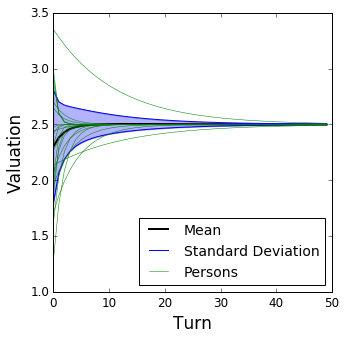
\includegraphics[width=6.5cm]{\fpath/f1.png}
  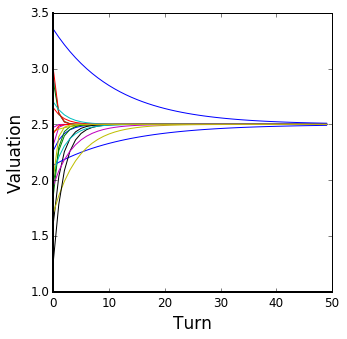
\includegraphics[width=6.5cm]{\fpath/f2.png}
  \caption{\small \textit{Each color represents the personal thinking of a person. For the simulation we set 1 restaurant, 20 persons and no friends; the restaurant capacity was set high enough to host all people.}}
  \label{fig:First_simulation}
\end{figure}

\begin{figure}[!htb]
	\centering
  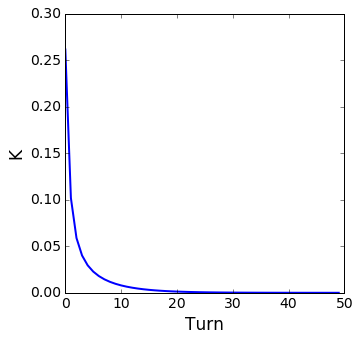
\includegraphics[width=7cm]{\fpath/f3.png}
  \caption{\small \textit{The $K$ coefficient for the simulation with 1 restaurant, 20 people, 50 turns and no friends}}
  \label{fig:First_simulation_k}
\end{figure}
As one can see from figure \ref{fig:First_simulation_k}, the $K_{re}$ coefficient after a sufficient number of turns converge to $0$, this means that at $t \to \infty$ all people will know the real quality of the restaurant $Q$.



\subsection{Second simulation: many restaurants}
\label{subsec:secon_exp}
In this second section we set-up simulations by considering a more realistic situation with many restaurants. Since people now have to choose where to go among many places, the way they take this choice becomes important. 

For all of this section's simulations, we set the restaurants real quality to $2.5$, half of the evaluation range, to analyse some of the interesting differences of the choice strategies.

\subsubsection{Randomly choose}
People select randomly the place where to eat.

\begin{figure}[!htb]
  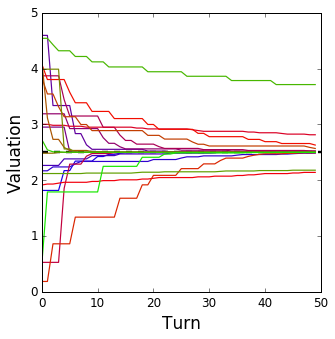
\includegraphics[width=6.5cm]{\fpath/rand1.png}
  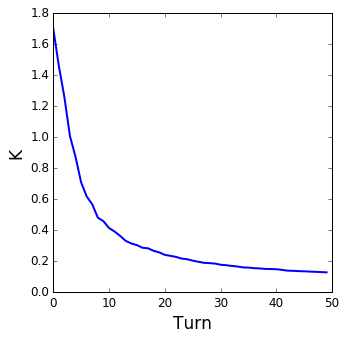
\includegraphics[width=6.5cm]{\fpath/rand2.png}
  {\small \textit{\caption{Simulation with:  4 restaurant, 20 persons, no friend, 50 turns, random choose.}}}
\end{figure}

In this case,  the process of updating the thinking is a bit different. Actually a person goes to different restaurants, and updates knowledge database only for that place; thus, since a person focuses only on a single restaurant we see that the curve is not an exponential but an exponential with some constant zones.
The process of discovering the real valuation is obviously slower than before.

\subsubsection{Person that chooses the best}
Every person tries to eat at the restaurant they thinks is the best. Thus, we observe that there are some restaurants that a person will never go to, and consequently will never updates his thoughts about them. This happens because each customer starts the simulation with a random valuation of every single restaurant. Thus there are people thinking from the beginning that the best restaurant in town is, instead, the worst one and they will never try something better. 
This situation may seems to be sensible if the restaurant is a really bad one, but would be ungodly if the restaurant is indeed a good one; in light of this, could happen that a good restaurant would be never discovered by someone just because the agent is convinced since the beginning (in real life, maybe because he heard about that) that the quality of it is really low. However, this issue could be resolved through the introduction of the communication among friends.
It also is to notice that the $K$ coefficient, in this case, seems not to converge to zero. This could be related to some of the evaluations remaining unchanged during the whole simulation.
\begin{figure}[!htb]
  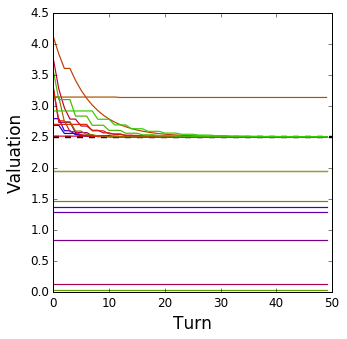
\includegraphics[width=6.5cm]{\fpath/best1.png}
  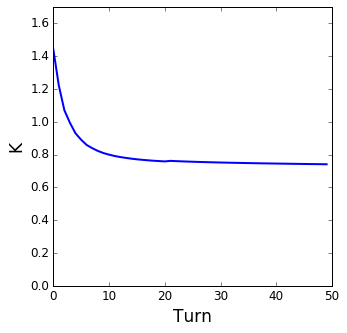
\includegraphics[width=6.5cm]{\fpath/best2.png}
  {\small \textit{\caption{Simulation with: 4 restaurant, 20 persons, no friend, 50 turns, best thinking choosing.}}}
\end{figure}

\pagebreak

\subsection{Third simulation: a bit more complicated}
\label{subsec:third_sim}
The simulations we considered until now are indeed too simple to reproduce a satisfying situation describing what happens in a real world; as a matter of fact, we could assume that people usually choose what they think is the best but we reasonably suppose that they will also explore the world. 
In this sense we introduce a bit more complex situation where we organize the probability of adopting a strategy instead of another in a different way: 50\% of time people goes to a restaurant randomly without considering its rank (\textit{irrational choose}) and  remaining 50\% of time they go to the one they think is the best choice.
\begin{figure}[!htb]
  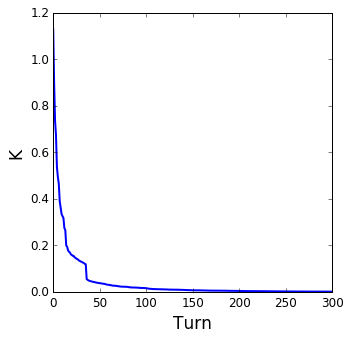
\includegraphics[width=6.5cm]{\fpath/50501.png}
  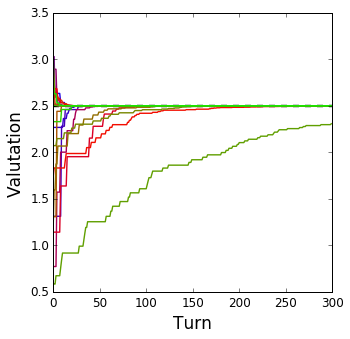
\includegraphics[width=6.5cm]{\fpath/50502.png}
  {\small \textit{\caption{Particular situation for a fixed restaurant. Simulation with: 4 restaurant, 20 persons, no friend, 300 turns, fifty-fifty strategy choice. All restaurants have ranking set to $2.5$.}}}
\end{figure}

Looking at the uncertainty factor $K_{re}$, introduced before, we observe that people are more incline in discovering new places even if they think, at first, they are not so good.
Moreover, in this case, we notice that people thought will converge to the real best restaurant, which rank is fixed to 2.5, faster than before and, furthermore, every person will convince itself that the best restaurant is indeed that one. 
This, simply means that more open-minded people, who are incline to try even places they don’t think are so good at first, will soon recognize which restaurant is the best one.



\subsection{Fourth simulation: communication among friends }
\label{subsec:friends}
In this section we start to introduce the communication among people. Thus, a person can communicate its thought to another. 
People base the choice of the restaurant again on both two strategies: the $50\%$ of turns they will adopt irrational choose, remaining ones they will go for best  choose.
Due to how we set the parameters in this simulation we obtain a more stochastic scenario because of the random choice (the 50\% of the time) and even produced by the fact that people could easily find a full restaurant; as a matter of fact the capacity of each place is finite.
In this sense, we need to make many different simulations that represent a single realization of the model.


\subsubsection{Many friends mean better choice}
In this subsection we deserved to study how the parameter $K$ changes in accord to the number of friends. We organize 4 different experiments incrementing the number of friends from 0 to 1,3 and 5 performing different realizations each.
In all experiment we set 20 people, 4 restaurants and 70 turns (time step conceived as 70 days).

Start considering the case with no friends. We plot $K(t)$ for all the 15 realizations of the experiment in  figure \ref{fig:15re}.
\begin{figure}[h]
  \centering
  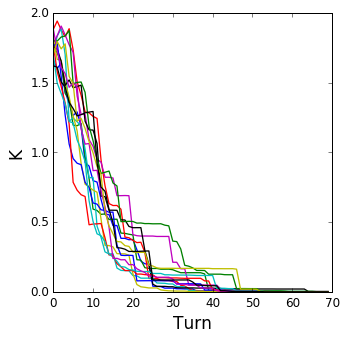
\includegraphics[width=9cm]{\fpath/Koverall.png}
  \caption{\small \textit{$K$ coefficient for the 15 simulations of this section. Each has been realized with 4 restaurants, 20 people, no friends for 70 turns}}
  \label{fig:15re}
\end{figure}
Then we compute the mean and the variance of $K(t)$ over all this different realizations (green curve) and try to approximate it with an exponential (red curve), as one can see from figure \ref{fig:aprox}.
\begin{figure}[h]
  \centering
  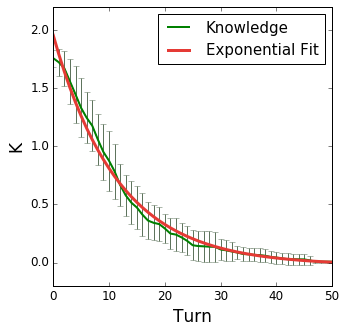
\includegraphics[width=9cm]{\fpath/koverallMean.png}
  \caption{\small \textit{$K$ coefficient mediated on the 15 simulations of the section (green line), with the corresponding exponential fit (red line)}}
  \label{fig:aprox}
\end{figure} 
The exponential regression is good as confirmed by a chi-square test.\\
$${\chi ^2} = 43.4 \text{ with } DF = 47$$
In particular the coefficients of the curve are:
\[K\left( t \right) = a{e^{ - bt + c}}\] 
\[\begin{array}{l}
a = 1.97\\
b = 0.086\\
c =  - 0.02
\end{array}\]
It can be interesting to consider the exponential \textit{time constant} $\tau  = \frac{1}{b} = 11.5$. This time constant can be interpreted as the number of turns needed to reduce $K$ by 63\% and approximately in $5 \tau = 57$ turns, the $K$ factor can be considered $0$, thus after 57 turns the global uncertainty is zero.

We reproduce the same analysis done with no friends by progressively increasing the number of friends as mentioned before.
Plotting the $K$ coefficient for all the different cases (figure \ref{fig:4curves}), we can see that for simulations with higher number of friends the $K$ factor converges to zero faster than scenarios with a lower number of friends, as shown in table \ref{tab:fit}. This is the consequence of the fact that people update more quickly their evaluation of restaurants by communicating with each other.  Thus, we observe that an higher number of friends leads to a faster convergence to the real quality.

\begin{figure}[!htb]
  \centering
  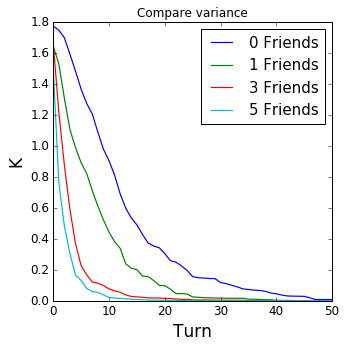
\includegraphics[width=9cm]{\fpath/varAmici.png}
  \caption{\small \textit{$K$ coefficient for simulations with 4 restaurants and 20 people with different number of friends, from 0 (blue line) to 5 (light blue line)}}
  \label{fig:4curves}
\end{figure}

\begin{table}[!htb]
\centering
\begin{tabular}{cccc}
\hline
number of friends & $b$ coefficient & $\tau$ & number of turns to zero \\ \hline
$0$ & $- 0.086$ & $11.5$ & $58$ \\ 
$1$ & $- 0.134$ & $7.4$ & $37$ \\ 
$3$ & $- 0.359$ & $2.7$ & $14$ \\ 
$5$ & $- 0.560$ & $1.8$ & $9$ \\ \hline
%\hline
%\rowcolor[HTML]{C0C0C0} 
%\multicolumn{1}{c}{\cellcolor[HTML]{C0C0C0}n friends} & $b$ coefficent                 & $\tau$                    & n turn to zero          \\ \hline
%\multicolumn{1}{|l|}{{\color[HTML]{333333} 0}}        & \multicolumn{1}{c|}{- 0.086}   & \multicolumn{1}{c|}{11.5} & \multicolumn{1}{c|}{58} \\ \hline
%\multicolumn{1}{|l|}{1}                               & \multicolumn{1}{c|}{- 0.134}   & \multicolumn{1}{c|}{7.4}  & \multicolumn{1}{c|}{37} \\ \hline
%\multicolumn{1}{|l|}{3}                               & \multicolumn{1}{c|}{- 0.359}   & \multicolumn{1}{c|}{2.7}  & \multicolumn{1}{c|}{14} \\ \hline
%\multicolumn{1}{|l|}{5}                               & \multicolumn{1}{c|}{- 0.560} & \multicolumn{1}{c|}{1.8}  & \multicolumn{1}{c|}{9}  \\ \hline
\end{tabular}
\caption{\small \textit{Comparison of fit parameter $b$ and time constant $\tau$ for the four experiments with increasing number of friends. It is also reported the number of turns the $K$ coefficient may be considered equal to zero}}
\label{tab:fit}
\end{table}

\pagebreak


\subsection{Average influx}
\label{subsec:avg_influx}

In this section we want to analyse the number of visits people made during the simulation to the restaurants.
We know that a person each turn goes to a restaurant according to the list of rankings stored in his knowledge database or chooses at random.
Hopefully, throughout the entire simulation every person will visit all restaurants at least once. 

One could think that, after an initial transient where the agents discover the world and progressively update their knowledge database with the effective quality of the restaurants, they will become more incline to visiting the best restaurant. 

To prove this, we set up a simulation with eight restaurants with rankings uniformly distributed over the entire range, from zero to
five, according to the rule 

\begin{equation*}
Q = \frac{2 n + 1}{2} \frac{5}{N}
\end{equation*}

where $Q$ is the restaurant's rank, $n$ is its index and $N$ is the total number of restaurants, equal to $8$. The resulting rankings are shown in table \ref{tab:ranks}.

\begin{table}[!htb]
\centering
\begin{tabular}{l | cccccccc}
\hline
$n$ & $0$ & $1$ & $2$ & $3$ & $4$ & $5$ & $6$ & $7$ \\ \hline
$Q$ & $0.31$ & $0.94$ & $1.56$ & $2.19$ & $2.81$ & $3.44$ & $4.06$ & $4.69$\\ \hline
\end{tabular}
\caption{\small \textit{Restaurant rankings for the influx simulations}}
\label{tab:ranks}
\end{table}

We considered thirty people who choose $50\%$ of time the best restaurant they can find and $50\%$ randomly. Each person also has $5$ friends to whom she sends her evaluations. We executed the simulation three times with different restaurant capacity.
In the first set-up the maximum capacity is set to $5$, then to $10$ and the last case has restaurants with maximum $15$ tables available each. 
For each set-up, we repeated the simulation five time in order to make some statistical considerations on the emerging behaviours. 

In light of this, we started considering one person at a time. We counted the times the same person goes to different restaurants during the entire simulation. Thus, we created an histogram with a bin per restaurant, ordered from the lowest rank to the highest one. On the vertical axis we counted the visits from the same person. We then mediated on all the people. 
%We also considered the total number of visits per turn for each restaurant.

\begin{figure}[!htb]
\centering
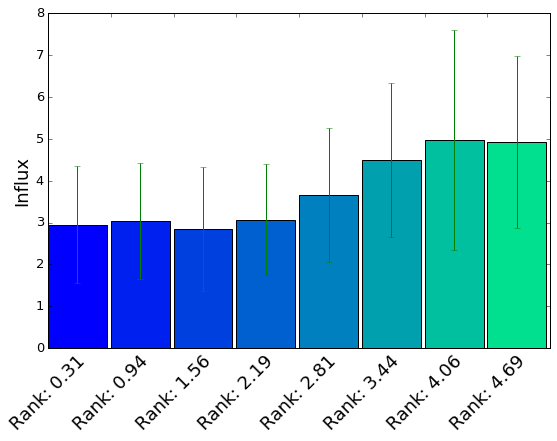
\includegraphics[width=7cm]{\fpath/5bis.png}
\caption{\small \textit{Results of the capacity $5$ simulation}}
\label{fig:Cap5R_isto}
\end{figure}

Figure \ref{fig:Cap5R_isto} shows the results of the first experiment with capacity $5$. As we could have foreseen, given the low capacity, many people will often find the best restaurants already filled and will then go to a lower ranked one. 
Besides, we observe that higher is the restaurant quality, higher will be the number of visits it receives.

Someone could notice that the restaurant number $6$ received an higher number of visits comparing number $7$. As we will better see later, the reason of this phenomenon could be related to two main factors. First of all if we consider a first transient period, where people do not know the real quality of each restaurant, they would easily go to a bad restaurant since maybe they are convinced it is the best one. The second motivation is linked to the choosing strategy that everyone adopts on each turn: as a matter of fact, when the $50\%$ of probability leads people to opt for a random choice, there is no reason they should to go to the best restaurant. This is why even worse restaurants receives a minimum number of visits.

Figure \ref{fig:Cap10R_isto} shows the next simulation, with capacity $10$. Given the higher capacity, more people will go to the best restaurant and the others will be gradually more empty.

\begin{figure}[!htb]
\centering
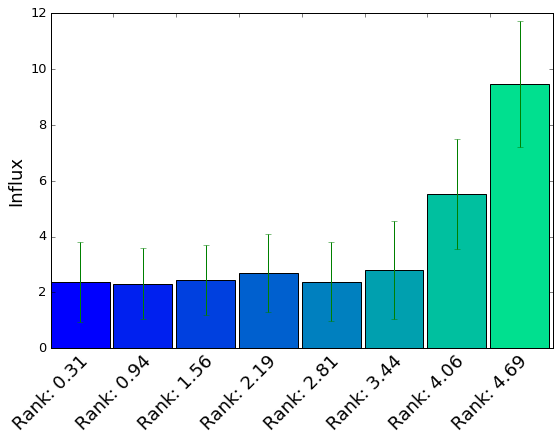
\includegraphics[width=7cm]{\fpath/10bis.png}
\caption{\small \textit{Results of the capacity $10$ simulation}}
\label{fig:Cap10R_isto}
\end{figure}

At last, figure \ref{fig:Cap15R_isto} shows the last simulation, with capacity $15$. Here, the trend we saw early is more strong.

\begin{figure}[!htb]
\centering
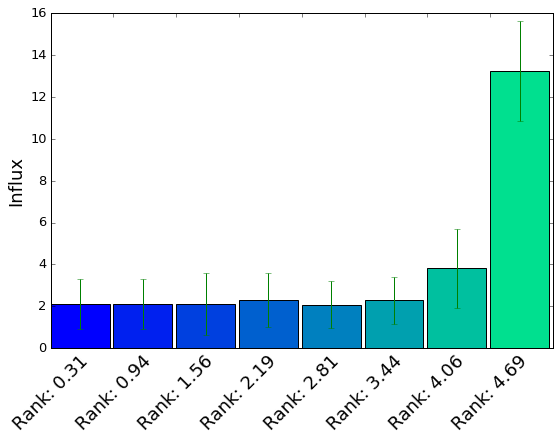
\includegraphics[width=7cm]{\fpath/15bis.png}
\caption{\small \textit{Results of the capacity $15$ simulation}}
\label{fig:Cap15R_isto}
\end{figure}

Nevertheless, there is one more unpredictable thing to outline. Looking at the figures, one can see that if the restaurant rank is lower than a certain value, it will always have some visits instead of being totally empty. In fact, the five worst restaurants usually always have the same number of visits within the error in each simulation.  This is much more evident when we increase the capacity.
To demonstrate this, we tested the compatibility of the worst restaurants' influx with a uniform law. Table \ref{tab:chi_perc} shows the results of the $\chi^2$ test, all confirming this hypothesis within the $5\%$ statistical significance.

\begin{table}[!htb]
\centering
\begin{tabular}{ccc}
\hline
capacity & D.o.F. & $\chi^2$\\ \hline
$5$ & $5$ & $3.7$\\
$10$ & $5$ & $2.56$\\
$15$ & $6$ & $5.97$\\ \hline
\end{tabular}
\caption{\small \textit{$\chi^2$ test results for the influx experiments}}
\label{tab:chi_perc}
\end{table}

This is probably related to the random choosing strategy, which creates a random noise responsible for this. Thus, no matter how bad a restaurant is, it will never be completely empty in a world where people  may choose randomly where to eat.

As for clarification, there are many factors that could lead people to go randomly in real life. For example one could think that a restaurant is really bad, and even though his friends are convinced of the contrary. Thus, not to break up the friendship, she will be obliged to go there, following the rest of the company. This is not a completely random choose in real life, but could be modelled that way in our MAS simulation.

\subsection{Percentage influx}
\label{subsec:perc_influx}

Focusing on all the restaurants instead of one person, we analysed the same simulations plotting the percentage of the population going to every restaurant each turn. 

Figure \ref{fig:Cap5R_time} shows the influx in time for the first simulation, with capacity $5$. One can observe that both the two top-ranked restaurants are always full after turn $5$. As we said before, in the first few turns takes place a transient where the people are still discovering the environment and updating their knowledge database. This phase explains the strange behaviour  we saw in figure \ref{fig:Cap5R_isto}, where the second best ranked restaurant recorded a slightly higher influx than the best one. As one can see from figure \ref{fig:Cap5R_time}, during the first few turns, the second best restaurant was slightly fuller than the best one, thus explaining the higher mean influx. 

\begin{figure}[!htb]
\centering
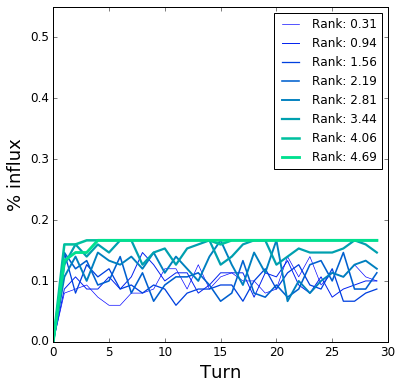
\includegraphics[width=7cm]{\fpath/5.png}
\caption{\small \textit{Influx in time for the capacity $5$ simulation}}
\label{fig:Cap5R_time}
\end{figure}

Figure \ref{fig:Cap10R_time} shows the influx in time for the second simulation, with capacity $10$. Given the higher capacity, the effect of the first transient is toned down and from the fifth turn most people go to the best-ranked restaurant. Because of the limited capacity value and the random choice behaviour, the worse ranked restaurants still record some influx later on the simulation.

\begin{figure}[!htb]
\centering
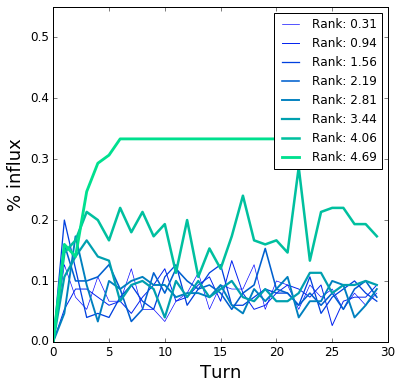
\includegraphics[width=7cm]{\fpath/10.png}
\caption{\small \textit{Influx in time for the capacity $10$ simulation}}
\label{fig:Cap10R_time}
\end{figure}

As one can see from figure \ref{fig:Cap15R_time}, which shows the influx in time for the capacity $15$ simulation, that the same trend already seen from figure \ref{fig:Cap15R_isto} is visible: people tend to fill the best restaurant, leaving the worst ones almost empty. The small influx recorded by those is due to the random choice strategy. Furthermore, we notice that the transient effect is much more attenuated.
One can also see that the best restaurant is almost never full. This is due to the high capacity, high enough to satisfy all the people who followed the rational strategy. Given a $50\%$ chance and thirty people, most times more than half may have chosen the random strategy, thus leaving the best restaurant not always full.

\begin{figure}[!htb]
\centering
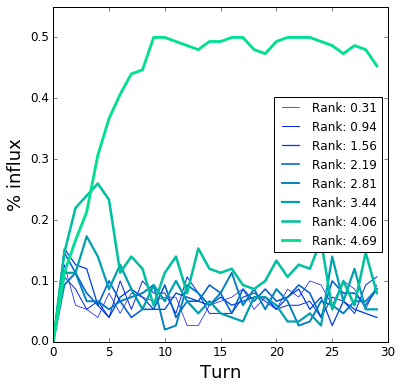
\includegraphics[width=7cm]{\fpath/15.png}
\caption{\small \textit{Influx in time for the capacity $15$ simulation}}
\label{fig:Cap15R_time}
\end{figure}

\subsection{Further considerations on strategy selection}
\label{subsec:further_considerations}

In previous sections we interpreted part of our results saying that some unpredictable phenomena were related to the fact that people could adopt two different strategies in the \textit{choose} phase of the
communication protocol: one that led them to choose random and another one, more rational, that takes them to the best restaurant. 

In order to better understand the weight that this random component  takes in our analysis, we remade the same simulations as before excluding the \textit{irrational choose} strategy. 
Thus, we expect not to have statistical fluctuations and to observe a more deterministic and rational collective behaviour.

\begin{figure}[!htb]
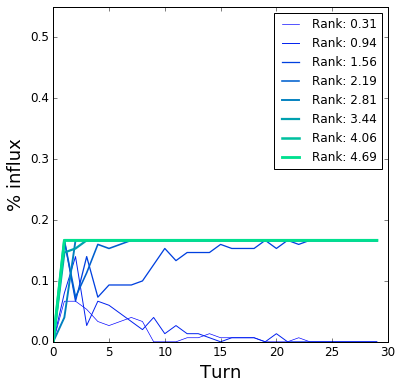
\includegraphics[width=7cm]{\fpath/NF5.png}
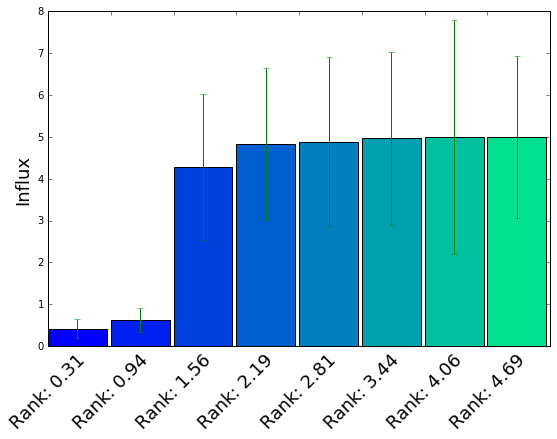
\includegraphics[width=7cm]{\fpath/5NFbis.png}
{\small \textit{\caption{Results for the capacity $5$ not random simulation}}}
\label{fig:Cap5NR}
\end{figure}

Figure \ref{fig:Cap5NR} shows the results for the first simulation, with capacity $5$. One can we immediately notice that this scenario is quite different than before. 
As one can see from the histogram, the two worst restaurants have a very little mean influx, due mostly to the initial transient. Given the low capacity, the other diners will be often full. 
Besides, looking at the second graph we have the confirmation that the trend is more deterministic. There are no longer statistical fluctuations since people always try to eat in the top-ranked diner which are progressively filled. It should also be noticed that the third worst restaurant takes quite all the simulation to be always completely full.

\begin{figure}[!htb]
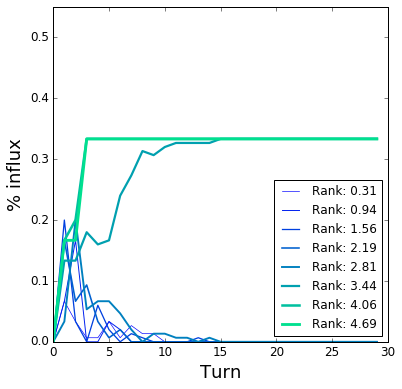
\includegraphics[width=7cm]{\fpath/NF10bis.png}
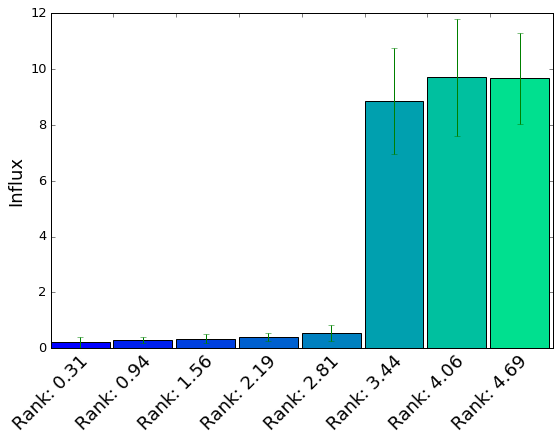
\includegraphics[width=7cm]{\fpath/NF10.png}
\caption{\small \textit{Results for the capacity $10$ not random simulation}}
\label{fig:Cap10NR}
\end{figure}

Figure \ref{fig:Cap10NR} shows the results for the capacity $10$ simulation. As one can see, in this case only the best three restaurants tend to be always full. This is due to the higher capacity, because the places available in three restaurants will be enough to host all of the thirty people considered for the simulation. As seen in the before, the worst diners are progressively emptier while people discover
there is something better in town.

Moreover, looking at the histogram, we have the confirmation that the only contribute to worst six restaurants is due to the initial transient. 

% plays an important
%role and outlines the ``intelligence'' of agents which trend is
%to explore the external environment adjourning their thought.

\begin{figure}[!htb]
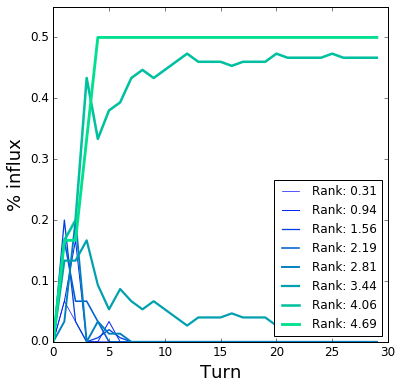
\includegraphics[width=7cm]{\fpath/NF15.png}
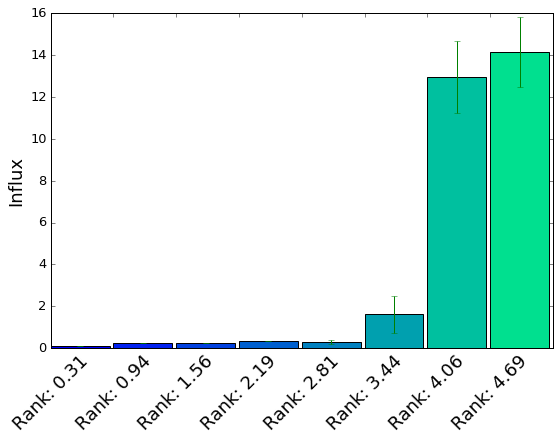
\includegraphics[width=7cm]{\fpath/NF15bis.png}
\caption{\small \textit{Results for the capacity $15$ not random simulation}}
\label{fig:Cap15NR}
\end{figure}

Figure \ref{fig:Cap15NR} shows the last simulation, with restaurant capacity $15$. One can see that, in this case, the two best restaurants are enough to satisfy the population's demand.

It is interesting to underline that the discovery of the environment is now much slower. One can notice that after $30$ turns there are people who still believe the third-ranked restaurant to be better than the second one. We could imagine that with a number of turns high enough, less people will go to worse restaurants and even the second-ranked diner will be filled as in the simulations previously showed. 

\section{Conclusions}
Finally, we conclude our work by remarking the most important results and behaviours we learnt from all the simulations we did in these sections.

First of all, in section \ref{subsec:eval_update_rule}, we analytically and, later, numerically verified that a person updates his knowledge database following an exponential law. Thus, even if it's thinking is initialized randomly he will converge to a real acquaintance of the world as a negative exponential.

Secondly, in section \ref{subsec:first_sim}, we moved to a first simulation with a single restaurant, a very simple case. Despite of this simplicity, we observed that all people involved in the simulation, notwithstanding their evaluation of the restaurant's quality was initialized randomly, converged at various speed to the consciousness of the objective quality of the only diner they could go to. In other words, this shows that our "dumb" agent progressively explores the environment by updating his own knowledge of the world towards a full understanding of what surrounds him.

Thirdly, we considered more than one restaurant, each with rating fixed at $2.5$: things became a bit more tricky since we started to consider different strategies on which a person agent could choose where to go. As explained in previous sections, we had a rational strategy and an irrational one. The first thing that we immediately noticed was that different strategies meant different convergence rate to a complete understanding of the environment. In this sense, we observed that the irrational choose strategy, which led people eat anywhere randomly, allows most of them to discover in about 50 turns the real quality of the restaurants. On the other hand, the rational way of choosing led to a much more slower process of discovery. Furthermore, because many were convinced since the beginning that the rank of some diners was lower than the real one, they never ate there, thus never modifying their evaluations. Because of that the variance did not converge to zero.

We then considered an hybrid situation of the two just discussed. We set the probability to choose each strategy at 50\% and the result, shown in section \ref{subsec:third_sim}, was that the convergence was much faster. Hence, we learnt that the best way to describe the people's process of discovery and exploration of the environment was to model their reasoning as half rational and half irrational. In this way a person agent will explore the environment and update his knowledge database to true values faster.

In section \ref{subsec:friends} we introduced the communication among friends and we discussed what happens when we increase the number of people communicating among themselves. Again, we found an exponential law. More precisely, in this case we numerically proved that the number of turns, the time constant $\tau$, required to fully discover the real rank exponentially decrease by increasing the number of friends, as shown in figure \ref{fig:4curves}. An explanation of this phenomenon could be that the informations spreads much faster if there are more people communicating and simultaneously discovering the environment.

Finally, in the last sections, we moved to the analysis of the average influx to diners from two different points of view: first we considered the people's point of view and then we computed the percentage influx in time for the restaurants' point of view. Despite at a first look it could seems to be a simple analysis we learnt something very interesting. In light of the considerations we made in section \ref{subsec:further_considerations}, the best way of simulating a real society is by introducing some fuzzy logic. For example, if we think at a situation where a town has eight restaurants of different qualities it is quite unrealistic to think that the three best-ranked will always be full while the others will always be empty. In this sense, as a last, important, consideration we could affirm that all what we learnt from our MAS model leads us to conceive the human behaviour as \textit{intrinsically irrational} as we need some non rational way of choosing (both sections \ref{subsec:avg_influx} and \ref{subsec:perc_influx}) to better reproduce the effects of human social behaviour.

\section{Further implementations}
It is important to remark that in these pages we exploited only a few of the entire potential that the MAS project we developed could have. Hence, we dedicate this last chapter to briefly introduce some further possible implementations, useful to extend the model, and other ideas that could help to make it much more powerful in analysing the human behaviour’s trend and more.

\subsection{Other parameters}
In this example we took in consideration, for what concerns people and restaurants, just a small number of parameters such as maximum evaluation, rank, capacity and so forth. We now want to discuss some other interesting features that we could introduce to have a more complete model that reproduces more faithfully what really happens in real life. In this sense, we could introduce:
\begin{itemize}
\item \textit{Price:} according to real life the price is a fundamental degree of freedom in the choosing of a diner. By not considering it, we simplified a lot our modelization of the social behaviours. For example, people could have a maximum price threshold they do not want to exceed in choosing the best diner. Similarly, restaurants would have an average price which tells how much should one spend on average by choosing that specific place.
\item \textit{Cooking type:} in the last years many ethnic and not conventional cuisine styles have diffused inside the alimentary culture in societies all around the world. For example, someone can eat a wonderful pizza in the center of Manhattan (even though, as we know, it is a typical Italian dish) or maybe prefers some Sushi in a typical Japanese restaurant around the corner of Alexanderplatz in Berlin. Because of that, it becomes natural to consider as another parameter to introduce in our model the cuisine type that a diner offers to customers. Obviously this will lead the model to a much more precise selection among the whole offer of all restaurants.
\item \textit{Position:} another important feature that could justify the choice of a diner instead of another is the position. When a person needs to eat somewhere maybe has no time to drive far, thus choosing some place nearby, in spite, for example, of the increasing price (e.g. central restaurants in town are much more expensive than suburban ones) or the quality. 
\item \textit{Alimentary exigency:} furthermore we can even think at allergies or particular exigences as parameters too. The most common one affect celiac people who need a very specific kind of cuisine in order to not have dangerous allergic reactions. Less problematic is the situation where people have exigences more related to a particular lifestyle instead of a disease such as vegan or vegetarian people.
\end{itemize}

As we can have insight, there is a really wide set of parameters to introduce in order to let the model become more and more precise and specific depending on the situations we're taking into account. For example, thinking at a situation where we consider only high quality restaurants in a wide geographic range, we could introduce as a new parameter the number of Michelin Stars each diner holds.

\subsection{Other strategies}
After looking at possible other parameters to implement, we now concentrate on the type of strategies that someone could adopt in choosing a restaurant. In our model we took in account just two of these: \textit{Choose the Best} and \textit{Irrational Choose}. 

As other examples, we could include:

\begin{itemize}
\item \textit{Weighted Irrational Choose:} this kind of strategy is a sort of crossover between the two we studied in section \ref{subsec:secon_exp}. This means that the person agent chooses randomly, but weighting how much is she disposed to risk finding a bad restaurant. To be more clear, a person is minded to go randomly but weighting the choice on the whole set of parameters that he has to take in account. Practically, she would weight with an utility function, calculated from the parameter set of each restaurant, the probability to choose one of them.

Another take on this strategy could be to compute the  utility function after the random choice, evaluating whether or not its value exceeds a certain risk threshold. If so, the person could randomly select another restaurant until she finds one risk-worthy.

%set a threshold and a weight for each parameter in the model. 
%
%When a person chooses a restaurant at random we multiply the weight of
%
%parameter i with the difference between the minimum value a person would accept
%
%for the i­esimo parameter and the value that the restaurant has. Than we sum up
%
%all these quantities for every degree of freedom (parameter) and if this value
%
%exceeds the threshold the choice is discard and the agent goes back to the search
%
%phase, otherwise he will opt for that restaurant. In this case people would sacrifice
%
%something (e.g. quality) in spite of something else (e.g. lower price) depending on
%
%the importance he gives to each one of the parameters (weight).

\item \textit{Best Friend Choose:} this is a very interesting strategy, useful to outline the influence of the communication between people in our model. In this strategy, a person decides to go to the restaurant which is thought the best one by the friend in which he believes the most (actually, his best friend!). In case this restaurant is already fully booked, it could be applied recursively to the second best restaurant in her friend's opinion and so on.
\end{itemize}

\subsection{Other fields of implementation}
The field this model has been applied to could also change. As a matter of fact, this work-flow and communication protocol is really powerful and could be generalized and adapted to a wide range of other domains. For example, we could simply consider hotels or travels instead of restaurants. We would certainly have different parameters but the basic reasoning would be the same. Moreover, this model could also be applied to predict the best choice for a specific customer in base of her needs and preferences.

\bibliographystyle{plainnat}
\bibliography{relazione}

\end{document}